%\documentclass[eng,final, oneside, printmode]{mgr} %mwbk
\documentclass[pl,final,oneside]{mgr} %printmode
\usepackage[polish]{babel}
\usepackage{polski}
\usepackage[OT4]{fontenc}
\usepackage[utf8]{inputenc}
\frenchspacing

\usepackage{cmap}
\linespread{1.1} %interlinia
\usepackage{amsmath}
\usepackage{amsfonts}
\usepackage{latexsym}
\usepackage{longtable}
\usepackage{graphicx} 
\usepackage{geometry}
\usepackage{pgfplots}
\usepackage{multirow}
\setlength{\parindent}{0pt}
\setlength{\parskip}{1ex plus 0.5ex minus 0.2ex}
\pgfplotsset{compat=1.13}
\usepackage{bookmark}
\usepackage{listings}
\usepackage{indentfirst}
\setcounter{secnumdepth}{6}

\usepackage[nottoc,numbib]{tocbibind}

\setlength{\parindent}{30pt}

\setlength{\parskip}{0pt}

\bookmarksetup{
	open,
	addtohook={%
		\ifnum\bookmarkget{level}<1 %
		\bookmarksetup{bold}%
		\fi
	},
}

\hypersetup{%
	colorlinks = true,
	linkcolor  = black
}

%\newgeometry{tmargin=1.5cm, bmargin=1.5cm, lmargin=1.5cm, rmargin=1.5cm}

% Default fixed font does not support bold face
\DeclareFixedFont{\ttb}{T1}{txtt}{bx}{n}{9} % for bold
\DeclareFixedFont{\ttm}{T1}{txtt}{m}{n}{9}  % for normal

% Custom colors
\usepackage{color}
\definecolor{deepblue}{rgb}{0,0,0.5}
\definecolor{deepred}{rgb}{0.6,0,0}
\definecolor{deepgreen}{rgb}{0,0.5,0}

\usepackage{listings}

% Python style for highlighting
\newcommand\pythonstyle{\lstset{
		language=Python,
		basicstyle=\ttm,
		otherkeywords={self},             % Add keywords here
		keywordstyle=\ttb\color{deepblue},
		emph={MyClass,__init__},          % Custom highlighting
		emphstyle=\ttb\color{deepred},    % Custom highlighting style
		stringstyle=\color{deepgreen},
		frame=tb,                         % Any extra options here
		showstringspaces=false,
		tabsize=3,
		%numbers=left,
		breaklines=true  % 
}}


% Python environment
\lstnewenvironment{python}[1][]
{
	\pythonstyle
	\lstset{#1}
}
{}

% Python for external files
\newcommand\pythonexternal[2][]{{
		\pythonstyle
		\lstinputlisting[#1]{#2}}}
% Python for inline
\newcommand\pythoninline[1]{{\pythonstyle\lstinline!#1!}}

%\renewcommand\lstlistingname{Dodatek A - spis listingów}
%\renewcommand\lstlistlistingname{{Dodatek A - spis listingów}}

\author{Rafał Dziwiński}
\title{Analiza możliwości i implementacja niezawodnego routingu w wirtualnym środowisku High Avability przy wykorzystaniu platformy Kubernetes oraz Calico.}

\engtitle{Analysis of possibilities and implementation of reliable routing in the virtual High Avability environment using the Kubernetes and Calico platforms.}
\supervisor{dr inż. Waldemar Grzebyk, KTT}
\field{Telekomunikacja}
\specialisation{Teleinformatyka i multimedia}

% \renewcommand*\thesection{\arabic{section}.} % zmiana numeracji sekcji 0.X -> X
\begin{document}

\maketitle
\tableofcontents

\chapter{Wstęp}
W dzisiejszych czasach... blablabla (wstęp i cel)
\chapter{Cel i zakres pracy}
Aspekt badawczy:
1. Opracowanie zakresu analizy oraz kryteriów oceny.
2. Analiza możliwości implementacji niezawodnego routingu w wirtualnym środowisku High Avability przy
wykorzystaniu platformy Kubernetes oraz Calico:
a) analiza sposobów implementacji niezawodnego routingu w środowisku wirtualnym,
b) porównanie rozwiązania zwirtualizowanego do fizycznego w oparciu o przyjęte kryteria.
Aspekt inżynierski:
1. Przygotowanie środowiska testowego wykorzystującego platformę Kubernetes oraz implementacja wirtualnych
routerów jako kontenerów przy pomocy aplikacji Docker.
2. Przygotowanie scenariuszy i procedur testowych.
3. Przeprowadzenie testów dotyczących czasu odzyskania pełnej funkcjonalności sieci w momencie awarii jednego
bądź wielu z jej elementów.
Zadania do wykonania:
1. Studia literaturowe.
2. Opracowanie zakresu analizy oraz kryteriów oceny.
3. Analiza możliwości implementacji niezawodnego routingu w wirtualnym środowisku High Avability przy
wykorzystaniu platformy Kubernetes oraz Calico:
a) analiza sposobów implementacji niezawodnego routingu w środowisku wirtualnym,
b) porównanie rozwiązania zwirtualizowanego do fizycznego w oparciu o przyjęte kryteria.
4. Przygotowanie środowiska testowego wykorzystującego platformę Kubernetes oraz implementacja wirtualnych
routerów jako kontenerów przy pomocy aplikacji Docker.
5. Przygotowanie scenariuszy i procedur testowych.
6. Przeprowadzenie testów dotyczących czasu odzyskania pełnej funkcjonalności sieci w momencie awarii jednego
bądź wielu z jej elementów.
7. Opracowanie wniosków z przeprowadzonej analizy i testów.
\chapter{Część teorytyczna}
BlaBlaBla
\section{Słownik pojęć}
\begin{description}
\item[Pod] najmniejsza możliwa do wdrożenia jednostka obliczeniowa zarządzana przez platformę Kubernetes.
\item[Node] maszyna robocza zawierająca usługi niezbędne do uruchamiania podów oraz zarządzania nimi.
\item[Master nod] maszyna robocza zapewniająca płaszczyznę sterowania klastra.
\item[Worker node] maszyna robocza zapewniająca zasoby sprzętowe dla tworzonych podów.
\item[Host endpoint] reprezentuje jeden bądź wiele fizycznych bądź wirtualnych interfjesów połączonych z hostem na którym uruchomione jest calico.
\item[Workload endpoints] reprezentuje zasób wirtualny podłączony do sieci Calico.
\item[Control plane] descriptioncontrol plane   aadsaef
\end{description}
\section{Konteneryzacja}
Konteneryzacja
Aby opisać w dobry sposób konteneryzację warto przypomnieć sobie jak było kiedyś. Pierwszą metodą wdrażania aplikacji było uruchomienie każdej z nich na osobnym fizycznym serwerze. Niestety, w tym przypadku nie ma możliwości wydzielenia zasobów dla danej aplikacji co powoduje problemy z jednoczesnym uruchomieniem wielu aplikacji. Może się zdażyć tak, że duże obciążenie na przykład przez atak DDoS spowoduje zatrzymanie pracy innych, zupełnie niezwiązanych ze sobą usług. Jedynym wyjściem jest uruchomienie aplikacji na osobnych fizycznych maszynach jednak generuje to szereg problemów. Między innymi:
\begin{itemize}
	\item Trudność w skalowaniu zasobów;
	\item zwiększenie ilości niewykorzystanych zasobów;
	\item duże koszty.
\end{itemize}
Aby temu zaradzić wprowadzono pojęcie wirtualizacji. Pozwala ona na uruchomienie wielu wirtualnych maszyn (VM) na jednym fizycznym serwerze. Pozwala to na izolację aplikacji co ma wpływ na stabilność w przypadku przeciążenia jednej z aplikacji oraz bezpieczeństwo. Kolejnym plusem jest możliwość lepszego zarządzania oraz skalowania zasobów sprzętowych.  Zmniejsza również koszt wdrożenia oraz utrzymania dzięki możliwości zastosowania jednego, wydajnego serwera oraz ograniczenie kosztu prądu. W tym przypadku każda z VM wirtualizuje fizyczne zasoby oraz sprzęt co również nie jest rozwiązaniem w stu procentach wydajnym.

Na pomoc przychodzi tak zwana konteneryzacja. Jest to rozwiązanie podobne do maszyn wirtualnych z tą różnica, że nie jest potrzebna wirtualizacja sprzętu oraz systemu operacyjnego. Kontener działa na jądrze systemu hosta oraz jego zasobach które nie są wirtualizowane. Oznacza to, że w przypadku wdrożenia aplikacji w kontenerze potrzebne jest jedynie dodanie do niego pakietów charakterystycznych dla tej aplikacji. Na przykład w momencie uruchomienia dystrybucji Fedora na fizycznym serwerze z Debianem kontener będzie zawierał jedynie pakiety charakterystyczne dla tej pierwszej dystrybucji. W ogromnych skrócie można powiedzieć, że jest to lżejsza wersja VM. Ponadto użycie kontenerów niesie za sobą wiele zalet:
\begin{itemize}
	\item Większa łatwość i wydajność tworzenia obrazu kontenera w porównaniu do użycia obrazu VM.
	\item Łatwiejszy rozwój aplikacji przez możliwość szybkiego budowania kolejnych obrazów.
	\item Możliwość łatwiej migracji między wieloma różnymi usługami w chmurze.
	\item Centralne monitorowanie oraz zarządzanie konternerami.
	\item Wydajniejsze oraz efektywniejsze zarządzanie zasobami sprzętowymi.
	
\end{itemize}
Różnicę między tradycyjnym wdrażaniem aplikacji a VM oraz kontenerami najlepiej obrazuje i podsumowuje poniższa grafika: 
\begin{figure}[h!]
	\centering
	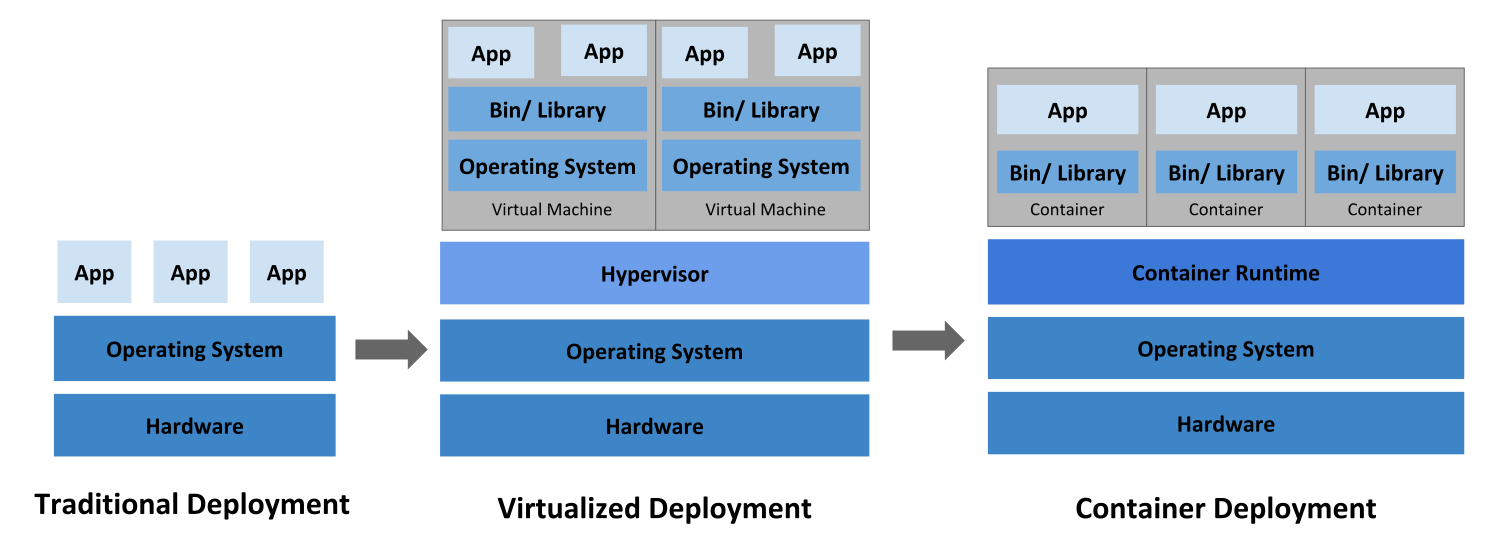
\includegraphics[width=1\linewidth]{images/container_evolution}
	\caption{Ewolucja możliwości wdrażania aplikacji \cite{kube_doku}.}
	\label{fig:container_evolution}
\end{figure}
\section{Kubernetes}
Słowo Kubernetes wywodzi się z języka greckiego i oznacza sternika bądź pilota. Pierwsze linie kodu napisane przez Google Inc. pojawiły się już w 2004 roku. Platforma bazuje na wieloletnim doświadczeniu tej firmy oraz społeczności.

Jest to otwarta platforma służąca do zarządzania skonteneryzowanymi aplikacjami oraz usługami. Głównym jej celem jest ułatwienie i automatyzacja ich wdrożeń oraz konfiguracji. Obecnie społeczność oraz firmy stojące za rozwojem systemu są na tyle liczne, że z powodzeniem ta młoda platforma może być wdrażana w środowiskach produkcyjnych.

Jak wspomniano w poprzednim rozdziale najlepszym z rozwiązań do uruchamiania aplikacji są kontenery. W środowisku produkcyjnym, liczącym wiele dziesiątek bądź też setek kontenerów    ręczne zarządzanie nimi jest niewydajne i obarczone ryzykiem wielu błędów. Również w momencie awarii konieczna jest szybka reakcja na przykład poprzez utworzenie zastępczych kontenerów. W tym celu bardzo dobrym wyjściem jest zastosowanie tak zwanego orkiestratora jakim jest Kubernetes. Do wymienionych wyżej zalet możemy dołączyć:

\begin{itemize}
	\item Wykrywanie usług oraz load balancing;
	\item automatyczne montowanie wybranych typów pamięci takich jak pamięć lokalna bądź zasób sieciowy;
automatyczne przydzielanie zasobów sprzętowych dla każdego z kontenerów;
	\item możliwość samoczynnego restartowania kontenera w momencie wykrycia awarii;
	\item łatwe zarządzanie danymi poufnymi wykorzystywanymi w kontenerach oraz zarządzanie ich konfiguracją.
\end{itemize}

\subsection{Komponenty}
W momencie wdrażania systemu Kubernetes nie uruchamiana jest pojedyncza aplikacja a szereg połączonych ze sobą usług. Aby to zrobić potrzebny jest tak zwany klaster składający się z minimum dwóch węzłów (node):
\begin{itemize}
	\item Worker node na której uruchamiane są kontenery 
	\item Master node zarządzający worker nodami oraz kontenerami w klastrze.
\end{itemize}
Przykładowy klaster wraz z wyszczególnionymi nodami został zaprezentowany poniżej.
\begin{figure}[h!]]
	\centering
	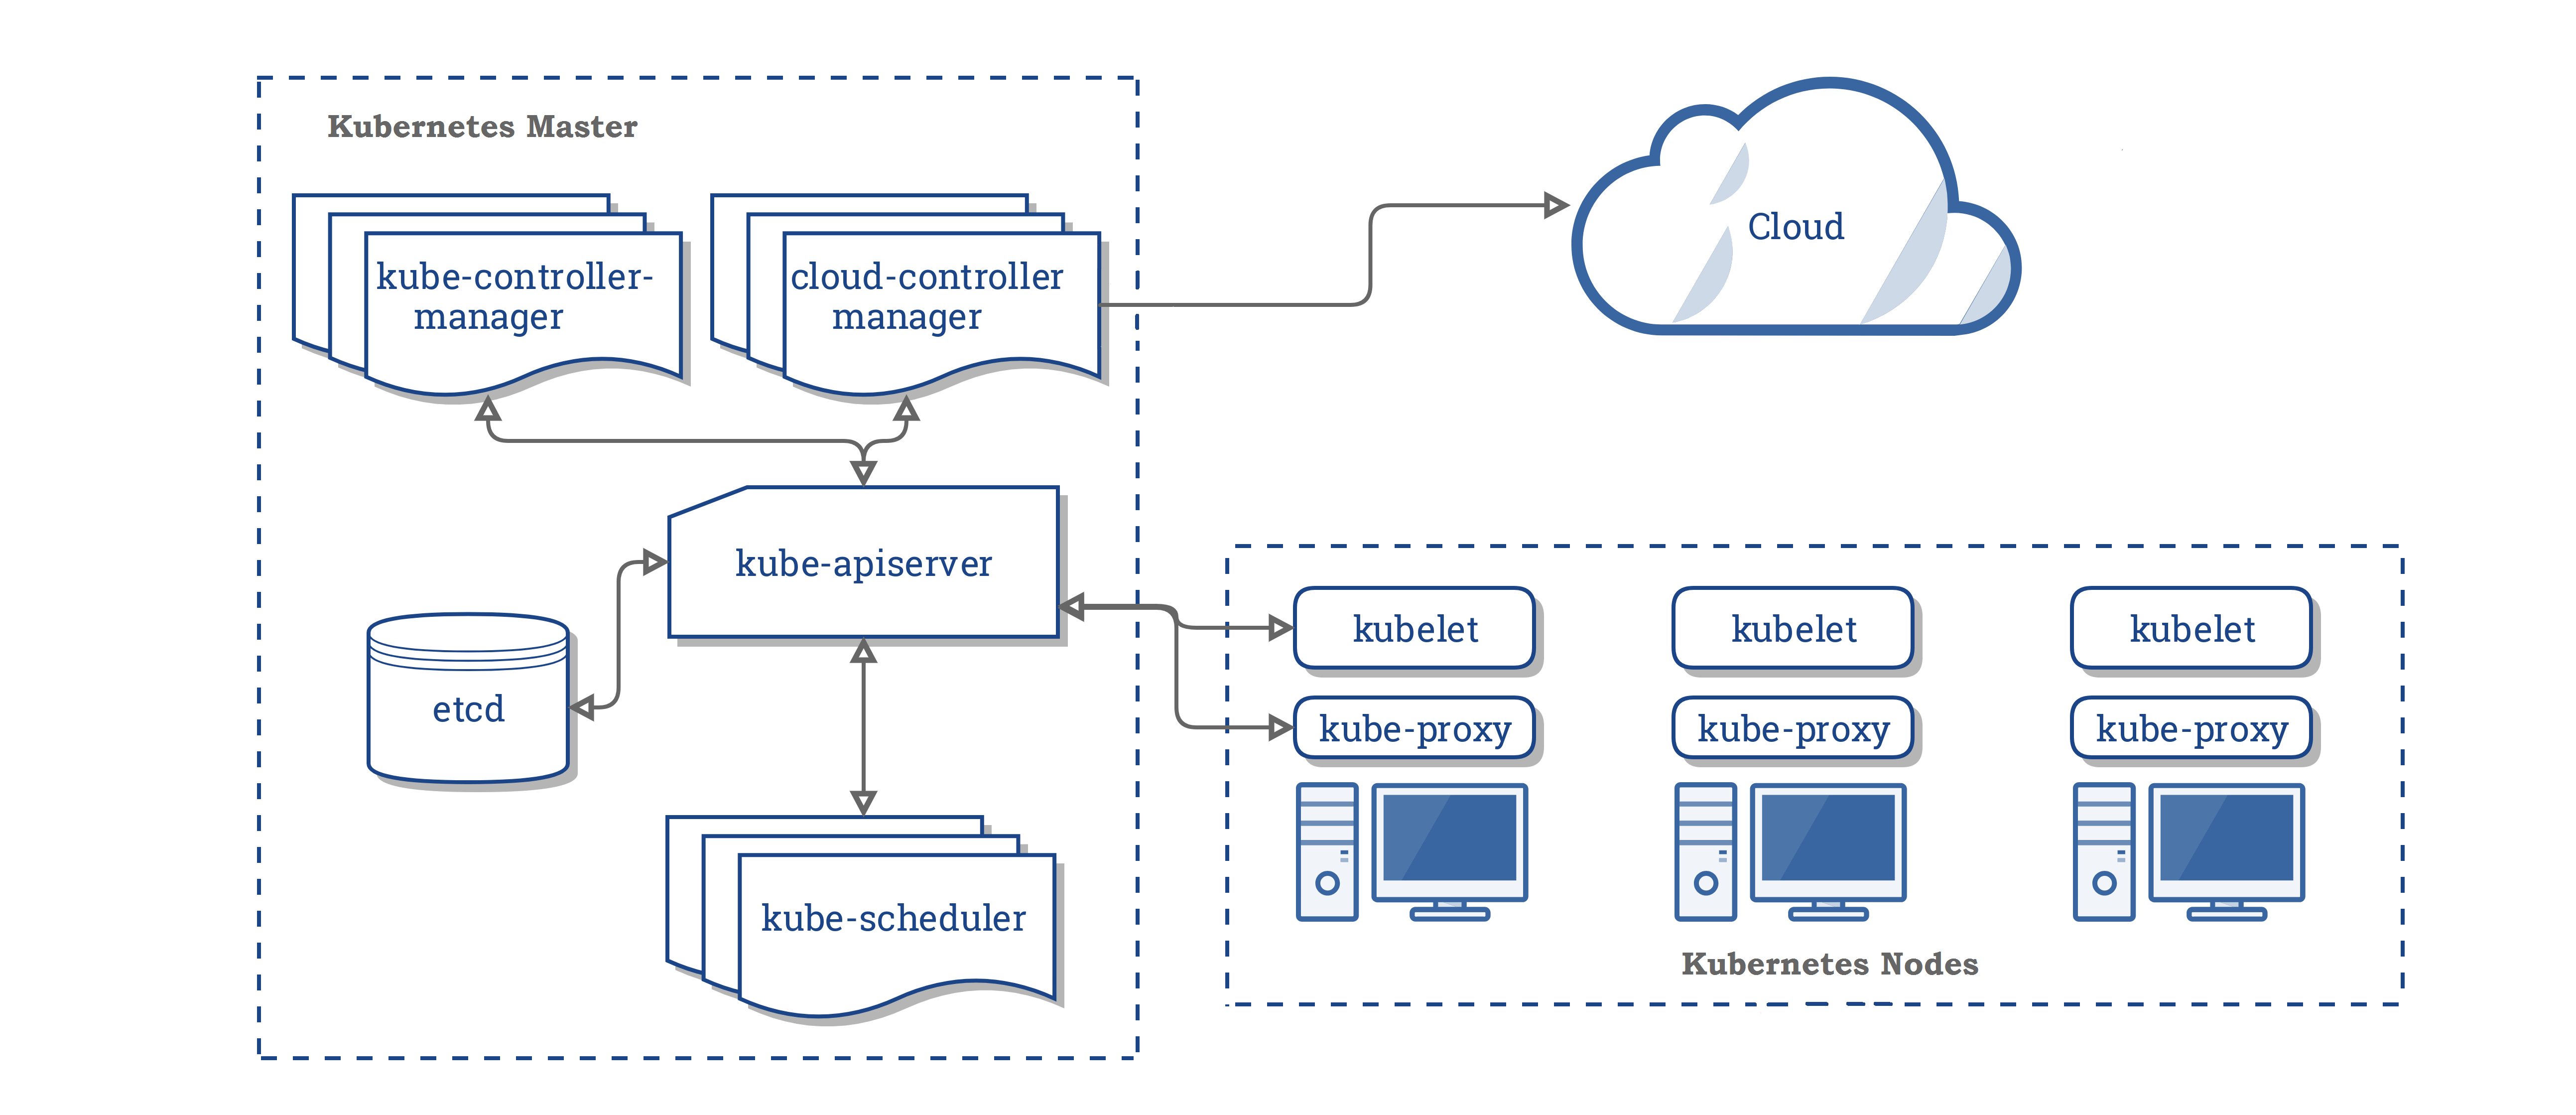
\includegraphics[width=1\linewidth]{images/components-of-kubernetes}
	\caption{Przykładowy klaster wraz z komponentami \cite{kube_doku}.}
	\label{fig:components-of-kubernetes}
\end{figure}

\subsubsection{Master Node}
Jak już wspomniano master node służy do zarządzania klastrem oraz kontenerami. Podejmuje on decyzje o umieszczeniu danego poda w node oraz zarządza ich zasobami. Składa się z szeregu komponentów które zostały wypisane oraz opisane poniżej:
\begin{description}
	\item [kube-apiserver] komponent control plane kubernetesa odpowiedzialny za komunikację użytkownika z platformą. 
	\item [etcd] silnie spójny i wysoce dostępny, rozproszony magazyn w formie klucz-wartość. Zapewnia niezawodny sposób przechowywaniakonfiguracji kubernetesa. Jeden z ważniejszych komponentów któremu konieczne jest zapewnienie nadmiarowości. Aby móc tolerować awarię jednego z modułów konieczne jest stworzenie klastra z ilością trzech.
	\item [kube-scheduler] komponent który w momencie wykrycia utworzenia nowego poda przypisuje go do odpowiedniego node bądź wielu. Decyzje te podejmuje na podstawie wymagań dotyczących zasobów/sieci poda oraz obciążenia obecnych workerów w klastrze. 
	\item [kube-controller-manager] komponent służący do uruchamiania kontrolerów. (https://kubernetes.io/docs/concepts/architecture/controller/) Każdy z kontrolerów jest osobnym procesem, lecz aby zwiększyć wydajnośc kompilowane są do jednego pliku binarnego. Zarządza on następującymi kontrolerami:
	\item [node controller] odpowiada za rekacje w momencie awarii jednego z node.
	\item [replication controller] zapewnia nadmiarowość podów w klastrze.
	\item [endpoints controller] zapewnia spójność usług oraz podów
	\item [service account and token controllers] tworzy użytkowników oraz zapewnia dostęp do API.
	\item [cloud-controller-manager] zapewnia integrację z siecią dostawcy usług chmurowych. 
\end{description}

\subsubsection{Node}
Poza kluczowymi komponentami wymienionymi w rozdziale wyżej które występują tylko w master node istnieją również dwa uruchamiane także na worker node.
\begin{itemize}
	\item kubelet - komponent którego zadaniem jest uruchamianie kontenerów wewnątrz podów. 
	\item kube-proxy - zarządza regułami sieciowymi w node pozwalającymi na komunikację podów z zasobami wewnątrz oraz poza klastrem. Jeżeli jest taka możliwość używa on zasoby oraz mechanizmy filtracji pakietów hosta.
	\item Container Runtime - komponent uruchamiający kontenery w klastrze. Na przykład: Docker, Containerd cri-o, bądź inny wspierany.
\end{itemize}



\section{Calico}
Calico jest to oprogramowanie wykorzystywane do zapewnienia sieci oraz jej bezpieczeństwa w środowiskach zwirtualizowanych oraz skonteneryzowanych. Jest ono otwarte i może być wykorzystywane przez wiele systemów takich jak OpenStack, OpenShift, Docker EE oraz Kubernetes. Głównymi założeniami twórców było stworzenie rozwiązania skalowalnego w środowiskach opartych o rozwiązania chmurowe oraz zapewnienie wydajności zbliżonej do rozwiązań oparty o jądro linuxa. Największymi zaletami Calico są:
\begin{itemize}
	\item Bezpieczeństwo - Użycie modelu “zero trust network” - wszystko co nie jest dozwolone jest zakazane.
	\item Wydajność - Calico korzysta z wbudowanych w jądro linuxa, wysoko zoptymalizowanych rozwiązań przekazywania oraz filtracji pakietów. W większości przypadków zbędne jest użycie funkcji enkapsulujących oraz dekapsulujących.
	\item Skalowalność - Osiągnięto ją dzięki wykorzystaniu najlepszych wzorców projektowych dla środowisk zwirtualizowanych oraz najpopularniejszych i najlepiej sprawdzonych protokołów sieciowych. Calico w cyklu testów deweloperskich jest uruchamiane na klastrze posiadającym wiele tysięcy node’s. 
	\item Uniwersalność - Poza zapewnieniem sieci dla systemów takich jak Kubernetes możliwe jest również wykorzystywanie w klasycznych maszynach wirtualnych a także interfejsach fizycznych.
\end{itemize}
\subsection{Host endpoints}
Calico poza możliwością definiowania punktów końcowych dla podów, maszyn wirtualnych bądź kontenerów umożliwia również tworzenie endpoints dla fizycznych interfejsów. Tak samo host endpoints może zawierać etykiety które znajdują się w tej samej przestrzeni nazw co workload endpoints. Calico nie wspiera konfiguracji adresów IP bądź konfiguracji w oparciu na adresach MAC interfejsów, zatem konieczna jest ich konfiguracja przez sieć podkładową naszego systemu.

Calico rozróżnia workload endpoints od host endpoints dzięki konfigurowalnym prefiksom. Dzięki polu  InterfacePrefix w konfiguracji modułu Felix możemy zdecydować, że punkty końcowe zaczynające się od danej wartości będą traktowane jako interfejsy workload. Pozostałe natomiast oznaczać będą interfejsy hosta.

Calico domyślnie blokuje cały ruch między workload interfaces, pozwalając tylko na ruch gdy interfejs jest znany oraz skonfigurowane są reguły bezpieczeństwa. W przypadku host endpoints Calico jest bardziej pobłażliwe. Monitoruje tylko ruch między zdefiniowanymi interfejsami, natomiast nie analizuje wszelkiego innego.

Możemy zastosować reguły bezpieczeństwa w kontekście punktów końcowych hosta dla trzech rodzajów ruchu:
\begin{itemize}
	\item zakończonego lokalnie,
	\item przekazywanego między host endpoints
	\item przekazywanego pomiędzy host endpoint a workload endpoint.
\end{itemize}
Przykład zastosowania wszystkich trzech rodzajów ruchu zaprezentowano na grafice poniżej;

\begin{figure}[h!]
	\centering
	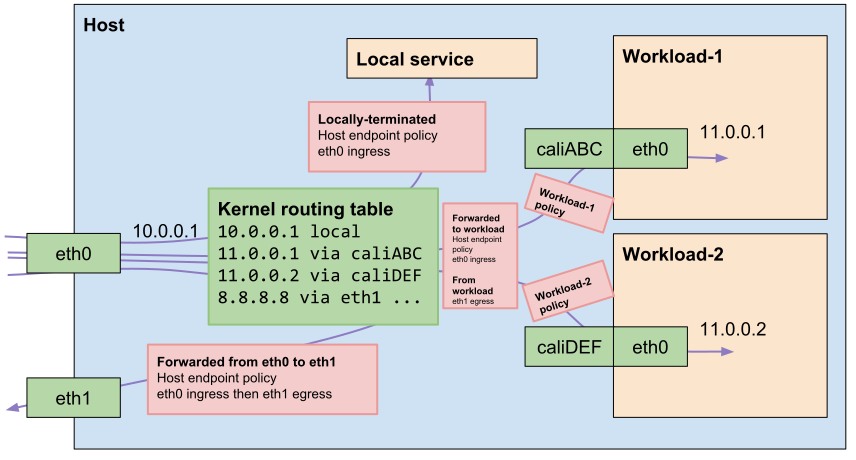
\includegraphics[width=1\linewidth]{images/bare-metal-packet-flows}
	\caption{Schmat pokazujący działanie calico w kontekście host endpoints \cite{calico_doku}.}
	\label{fig:bare-metal-packet-flows}
\end{figure}



\begin{thebibliography}{99}
	\bibitem{kube_doku} 
	Dokumentacja projektu Kubernetes,
	\\ \textit{https://kubernetes.io/docs/home/}
	
	\bibitem{calico_doku}
	Dokumentacja projektu Calico \\
	\textit{https://docs.projectcalico.org/v3.10/introduction/}

	\bibitem{kube_in_action} 
	Kubernetes in Action, Manning Publications 2017 \\
	\textit{ISBN: 9781617293726}
	
	\bibitem{kube_up_and_run} 
	Kubernetes: Up and Running, O'Reilly Media, Inc. 2017 \\
	\textit{ISBN: 9781491935675}
	
	\bibitem{docker_fundamentals}
	Learn Docker - Fundamentals of Docker 18.x, Packt Publishing 2018\\
	\textit{ISBN: 9781788997027}

\end{thebibliography}
\end{document}

